\documentclass[12pt]{article}
\usepackage{geometry}
\usepackage{amsmath}
\usepackage{array}
\usepackage{amsthm}
\usepackage{amsfonts}
\usepackage{ulem}
\usepackage{graphicx}
\usepackage{caption}
\usepackage{subcaption}


\geometry{a4paper,centering,scale=0.8}
\rmfamily
\normalsize
\setlength{\parindent}{0em}

\begin{document}
\begin{flushleft}
Junlong Gao 5133709126\\
Prof. Hohberger\\
Vv186\\
September 20, 2013\\%date
\end{flushleft}


\textbf{Exercise 1}\\
\textit{Solution:}\\
i) a) $(1,+\infty)$, $(-\infty,1]$; \\
b) $(1,+\infty)$, $(-\infty, -1]$;\\
c) $(0,+\infty)$, $(-\infty,0]$; \\
d)$[\sqrt{2},+\infty)$, $(-\infty, 0]$.\\

ii) First $X$ is bounded above,
then $\sup X$ exists,
thus  $y>\sup X$ is in $Y$,
thus it's non-empty.
Also, since for any $y\in Y$,
there exists $x\in X$ such that $y>x$,
all $y$ is bounded by $\inf X$,
that is, $Y$ is bounded below.\\

iii) a):$1$ b):$1$ c):$0$ d):$\sqrt{2}$

iv) Given $X$ is a bounded infinite set, let $Y=\{y\in R: x>y $ for all but finite many $ x\in X\}$,
then it's bounded above, then \textit{limit inferior} $:=\sup Y$\\
a):$1$ b):$-1$ c):$0$ d):$0$

v)\\
(a) Assume $\overline{\text{lim}}A < \uline{\text{lim}}A$,
then let $t=(\overline{\text{lim}}A +\uline{\text{lim}}A)/2$, giving $\overline{\text{lim}}A<t<\uline{\text{lim}}A$. We see that all $a\in A$ can be classified into $a>t$ and $a\le t$.
But there's only finite many $a$ satisfy that inequality by definition,
contradicts the fact that $A$ is infinite.\qed\\

(b) If $y$ is an almost upper bound, then $\overline{\lim}A\leq y$ ,
on the other hand, $\sup A$ is also an almost upper bound, so we have $\overline{\lim}A\leq\sup A$.\\
Similarly, if $y$ is an almost lower bound, then $\underline{\lim}A\ge y$ ,
on the other hand, $\inf A$ is also an almost lower bound, so we have $\underline{\lim}A\ge\inf A$.\qed\\

(c) Suppose we have $\overline{\text{lim}}A<$sup$A$,
then there exists $a\in A$ such that $(\overline{\text{lim}}A+\text{sup}A)/2\leq a\leq $sup$A$, 
let all that $a$ forms $A'$, 
and it's non-empty and finite according to the definition,
thus ${\max A=\max A'}$, which exists for finite sets.\\
Similarly, suppose we have $\uline{\lim}A>\inf A$,
then there exists $a\in A$ such that $(\underline{\lim}A+\text{inf}A)/2\ge a\ge \inf A$,
let all that $a$ forms $A''$, and it's non-empty and finite according to the definition, 
thus ${\min A=\min A''}$, which exists for finite sets.\qed\\

\textbf{Exercise 2}\\\
\textit{Proof: }\\i) Suppose $z_1=a+bi, z_2=c+di$, then we have:
\begin{alignat*}{6}
\quad\quad|z_1z_2|^2&=(ac-bd)^2+(ad+bc)^2\\
&={(ac)}^2+{(bd)}^2-2abcd+{(ad)}^2+{(bc)}^2+2abcd\\
&=a^2(c^2+d^2)+b^2(c^2+d^2)\\
&=(a^2+b^2)(c^2+d^2)\\
&={|z_1|}^2{|z_2|}^2
\end{alignat*}
Namely $|z_1z_2|=|z_1||z_2|$\\
ii) Let $z=a+bi$, where $a,b\in\mathbb{R}$
\begin{alignat*}{6}
&&|a+2+bi|&\leq|a-1+bi|\\
&\Longrightarrow \quad&{(a+2)}^2+b^2&\leq{(a-1)}^2+b^2\\
&\Longrightarrow &2a+1&\leq0\\
&\Longrightarrow & a&\leq-\frac{1}{2}
\end{alignat*}
So the desired set is $\{z:\Re(z)<-\frac{1}{2}\}$\\\
iii) \begin{alignat*}{6}
&   &(1+2i)z+(1-i)^2&=i-(2+i)z\\
&\iff\quad		  &(3+3i)z&=3i\\
&\iff     &z=\frac{i}{1+i}&=\frac{1+i}{2}
\end{alignat*}
iv) See the end of the paper.\\
v)
\begin{alignat*}{6}
{|z_1+z_2|}^2+{|z_1-z_2|}^2
&=(z_1+z_2)\overline{(z_1+z_2)}+(z_1-z_2)\overline{(z_1-z_2)}\\
&=(z_1+z_2)(\overline{z_1}+\overline{z_2})
+(z_1-z_2)(\overline{z_1}-\overline{z_2})\\
&=2z_1\overline{z_1}+2z_2\overline{z_2}\\
&=2\left({|z_1|}^2+{|z_2|}^2\right)
\end{alignat*}
\qed
\\
\textbf{Exercise 3}\\
\textit{Proof: }\\
i) Let $\epsilon>0$ be fixed,
let $N>1/\sqrt\epsilon$, if $n>N$, we have:
\[
\left|\frac{1}{n^2}-0\right|<\left|\frac{1}{N^2}\right|<\epsilon
\]
Thus 
\[
\lim_{n\to+\infty}\frac{1}{n^2}=0
\]\\
Let $\epsilon>0$ be fixed, let $N>5/\epsilon$, if $n>N$, we have:
\[
\left|\frac{2n-5}{n}-2\right|=\frac{5}{|n|}<\epsilon
\]
Thus 
\[
\lim_{n\to+\infty}\frac{2n-5}{n}=2
\]\\
ii) Let $\epsilon>0$ be fixed, 
then there exists  $N_1$ such that $n>N_1$ implies
\[
|b_n-b|<\frac{\epsilon}{2|a+1|}
\]
Also there exists $N_2$ such that $n>N_2$ implies
\[
|a_n-a|<\frac{\epsilon}{2|b|}
\]
Finally, there exists  $N_3$ such that $n>N_3$ implies
\[
|a_n-a|<1
\]
Thus we get
\[
|a_n|\leq|a_n-a|+|a|\leq1+|a|=|1+|a||
\]
By letting $N>$max$(N_1,N_2,N_3)$ we have:
\begin{align*}
|a_nb_n-ab|&<|a_n||b_n-b|+|b||a_n-a|\\
&<|a+1|\frac{\epsilon}{2|a+1|}+|b|\frac{\epsilon}{2|b|}\\
&=\frac{\epsilon}{2}+\frac{\epsilon}{2}=\epsilon
\end{align*}
\qed
\\
\textbf{Exercise 4}\\
\textit{Solution: }\\
For $a_n$:
\begin{alignat*}{6}
\lim_{n\to+\infty}a_n&=
\lim_{n\to+\infty}\frac{1-\frac{3}{n}
+\frac{2}{n^2}}{2+\frac{5}{n}+\frac{10}{n^2}}\\
\intertext{Limit plays nicely with algebra operation:}
&=\frac{1-\displaystyle\lim_{n\to+\infty}\frac{3}{n}
+\lim_{n\to+\infty}\frac{2}{n^2}}
{2+\displaystyle\lim_{n\to+\infty}\frac{5}{n}
+\lim_{n\to+\infty}\frac{10}{n^2}}\\
&=\frac{1}{2}
\end{alignat*}

For $b_n$:
\begin{alignat*}{6}
\intertext{Note that by \textit{Bernoulli's inequality}}
1-1/n=1-n^{-2}n&\leq b_n\leq 1-n^{-2}\tag{For $n\ge1$}
\intertext{Limits of both sides goes to 1, so by squeeze theorem:}
\lim_{n\to\infty}b_n&=1
\end{alignat*}

For $c_n$, we note that $n/m<1$ for $m>n$, thus
\[
0\leq\frac{n^n}{(2n)!}\leq \frac{1}{n!}
\]
Both sides goes to 0 as $n\to \infty$, 
so the squeeze theorem tell us that 
\[
\lim_{n\to \infty}c_n=0
\]

For $d_n$, since $n!$ has $n-1$ factors, 
excluding $1$, all of them are less than $n$, we obtain the inequality:

\[
0\leq\frac{n!}{n^n}\leq\frac{n^{(n-1)}}{n^n}=\frac{1}{n}
\]
Now by squeeze theorem and $1/n\to0$ as $n\to\infty$
\[
\lim_{n\to\infty}d_n=0
\]
For $e_n$,
\[
e_n=\frac{1}{\sqrt{n+1}+\sqrt{n}}
\]
We have
\[
\lim_{n\to\infty}e_n=
\frac{1}{\displaystyle\lim_{n\to\infty}\sqrt{n+1}+\sqrt{n}}=0
\]
Altogether, we have:
\[
\lim_{n\to\infty}a_n=\frac{1}{2};
\quad\lim_{n\to\infty}b_n=1;
\quad\lim_{n\to\infty}c_n=0;
\quad\lim_{n\to\infty}d_n=0;
\quad\lim_{n\to\infty}e_n=0.
\]
\\
\textbf{Exercise 5}\\
\textit{Proof: }\\
Let $\epsilon>0$ be fixed and given, 
then there exists $N_1$ such that $n>N_1$ and $n$ is odd implies:
\[
|a_n-a|<\epsilon
\]
Also there exists $N_2$ such that $n>N_2$ and $n$ is even implies:
\[
|a_n-a|<\epsilon
\]
Let $N>\max(N_1,N_2)$, 
then $\forall n>N$ is either even or odd,
satisfying $|a_n-a|<\epsilon$, thus $a_n\to a$ as $n\to \infty$
\qed
\\\
\\
\textbf{Exercise 6}\\
\textit{Proof: }\\i) Given $a_n=m/n$, then
\[
a_{n+1}=\frac{m+2n}{m+n}
=\frac{m/n+2}{m/n+1}
=\frac{a_n+2}{a_n+1}
=1+\frac{1}{1+a_n}
\]\qed

ii) Note $a_{2n}^2>a_{2n+2}^2>2$ 
after two transformation in Exercise 1 Assignment 8,
provided that $a_2^2>2$,
so it's monotonic and bounded by $a_2=3/2$,
since every monotonic and bounded sequence is convergent,
so $\{a_{2n}\}$ is converge. 
Finally, since $a_{2n}$ and $a_{2(n+1)}$ has the same limit $a$,
we have:
\[
\lim_{n\to \infty}a_{2(n+1)}=
\lim_{n\to\infty}1
+\frac{1}{1+a_{2n+1}}
=\lim_{n\to\infty}\frac{3a_{2n}+4}{2a_{2n}+3}
\]
That is
\begin{alignat*}{6}
&a=\frac{3a+4}{2a+3}\\
\Longrightarrow \quad&a^2=2\\
\end{alignat*}
Since all terms are strictly positive, then we have $a=\sqrt2$
\qed\\

iii) The proof is quite symmetry.
Note $a_{2n-1}^2<a_{2n+1}^2<2$
after two transformation in Exercise~1 Assignment~8,
provided that $a_1^2<2$,
so it's monotonic and bounded by 2,
since every monotonic and bounded sequence is convergent,
so $\{a_{2n-1}\}$ is converge. 
Finally, since $a_{2n-1}$ and $a_{2n+1}$ has the same limit $a$, we have:
\[
\lim_{n\to \infty}a_{2n+1}
=\lim_{n\to\infty}1+\frac{1}{1+a_{2n}}
=\lim_{n\to\infty}\frac{3a_{2n-1}+4}{2a_{2n-1}+3}
\]
That is
\begin{alignat*}{6}
&a=\frac{3a+4}{2a+3}\\
\Longrightarrow \quad&a^2=2\\
\end{alignat*}
Since all terms are strictly positive, then we must have $a=\sqrt2.$\\
Now by Exercise 5, we conclude that $a_n\to\sqrt 2$ as $n\to\infty$
\qed\\

iv) For given $\sqrt c=\sqrt{a^2+b}>1,a,b\in \mathbb{N}$ we define
\begin{align*}
&x_1=1
&x_{n+1}=a+\frac{b}{a+x_n}
\end{align*}
First we check boundaries:
\[
{x_{n+1}^2-c=
\left(\frac{ax_n+c}{a+x_n}\right)^2-c=
\frac{(c-a)(c-x_n^2)}{(a+x_n)^2}}
\]
That is, $x_n^2<c$ yields $x_{n+1}^2>c$ and vice versa.\\
Thus all odd terms are bounded above by $\sqrt c$,
all even terms are bounded below by $\sqrt c$

Next we check monotonity:
\[
x_{n+2}-x_{n}
=a+\frac{b}{a+a+\frac{b}{a+x_n}}-x_n
=\frac{2a(c-x_n^2)}{2a(a+x_n)+b}
\]
Since it's sign is determined by $(c-x_n^2)$,
all odd terms are monotonically increasing,
while all even terms are monotonically decreasing,
and every monotonic and bounded sequence is convergent,
thus both even and odd subsequence has a limit.\\
Finally, we observe that when n is odd, we have:
\[
0=\lim_{n\to\infty}x_{n+2}-\lim_{n\to\infty}x_n
=\lim_{n\to\infty}\frac{2a(c-x_n^2)}{2a(a+x_n)+b}
\]
Note that $2a(a+x_n)+b$ is bounded below by $b\ge 1$,
so we deduce that $x_n\to\sqrt c$ as odd $n\to\infty$,
same proof works when $n$ is even.\\
Thus the we have shown $x_n\to\sqrt c$ as $n\to\infty$,
namely the continued fraction expansion.
\qed\\


\textbf{Exercise 7}\\
\textit{Proof: }\\
i) First we observe that
\[
a_{n+1}^2-b_{n+1}^2=\frac{{(a_n-b_n)}^2}{4}>0
 \tag{$n\in\mathbb{N}$}
\]
Similarly $a_1\ge b_1$\\
Then
\begin{alignat*}{6}
a_{n+1}-a_n&=\frac{b_n-a_n}{2}<0\\
b_{n+1}-b_n&=\sqrt{b_n}(\sqrt{a_n}-\sqrt{b_n})>0
\end{alignat*}
And $a_n$ is bounded below by 0,
$b_n$ is bounded above by $a_n$,
or $a_1$, we claim each of them must converge.\\
Note that we have $a_n>b_n$ thus $\sqrt{a_nb_n}>b_n$, 
\[
0\leq|a_{n+1}-b_{n+1}|=\frac{a_n+b_n}{2}-\sqrt{a_nb_n}<\frac{a_n+b_n}{2}-b_n=\frac{|a_n-b_n|}{2}\leq\frac{a_1-b_1}{2^n}
\]
By squeeze theorem,$\displaystyle\lim_{n\to\infty}|a_n-b_n|=0$, namely
\[
\lim_{n\to\infty}a_n=\lim_{n\to\infty}b_n
\]
\qed
\\
ii) First we observe that
\[
a_{n+1}-b_{n+1}
=\frac{{(a_n-b_n)}^2}{2(a_n+b_n)}>0 \tag{$n\in\mathbb{N}$}
\]
Similarly $a_1\ge b_1$\\
Then
\begin{alignat*}{6}
a_{n+1}-a_n&=\frac{b_n-a_n}{2}<0\\
b_{n+1}-b_n&=\frac{b_n(a_n-b_n)}{a_n+b_n}>0
\end{alignat*}
And $a_n$ is bounded below by 0,
$b_n$ is bounded above by $a_n$,
or $a_1$, thus we claim each of them must converge.\\
Note that $a_n>b_n$,we have
\[
b_{n+1}=\frac{2a_nb_n}{a_n+b_{n}}>\frac{2a_nb_n}{a_n+a_n}=b_n
\]

Thus
\[
0\leq|a_{n+1}-b_{n+1}|=\frac{a_n+b_n}{2}-\frac{2a_nb_n}{a_n+b_{n}}
\frac{a_n+b_n}{2}-b_n=\frac{a_n-b_n}{2}\leq\frac{a_1-b_1}{2^n}
\]
By squeeze theorem,$\displaystyle\lim_{n\to\infty}|a_n-b_n|=0$, namely
\[
\lim_{n\to\infty}a_n=\lim_{n\to\infty}b_n=HG(a,b)
\]
Where $HG(a,b)$ stands for the {\it arithmetic-harmonic mean}.

Finally, we notice that:
\begin{alignat*}{6}
a_{n+1}b_{n+1}=\frac{a_n+b_n}{2}&\frac{2a_nb_n}{a_n+b_n}
=a_nb_n=ab
\intertext{Taking the limit, we obtain}
{HG}^2(a,b)&=ab\\
\intertext{That is:}
HG(a,b)&=\sqrt{ab}
\end{alignat*}
\eject
\begin{figure}
        \centering
        \begin{subfigure}[b]{0.5\textwidth}
                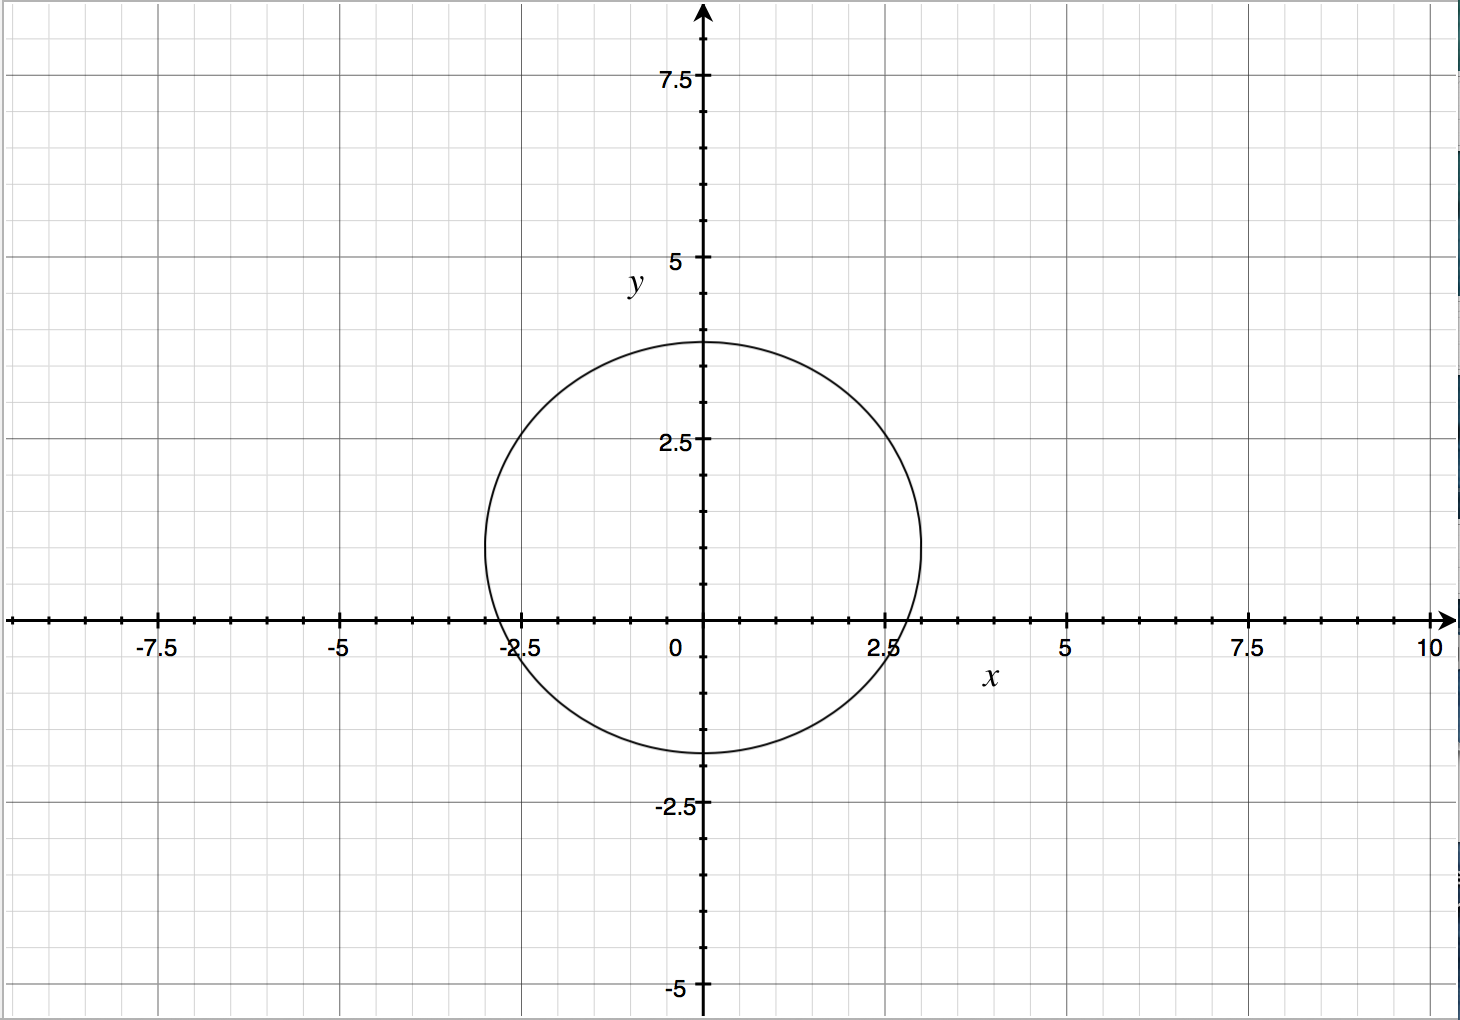
\includegraphics[width=\textwidth]{A.eps}
                \caption{Ellipse Centered at $(0,1)$}
                \label{fig:gull}
        \end{subfigure}%
        ~ %add desired spacing between images, e. g. ~, \quad, \qquad etc.
          %(or a blank line to force the subfigure onto a new line)
        \begin{subfigure}[b]{0.5\textwidth}
                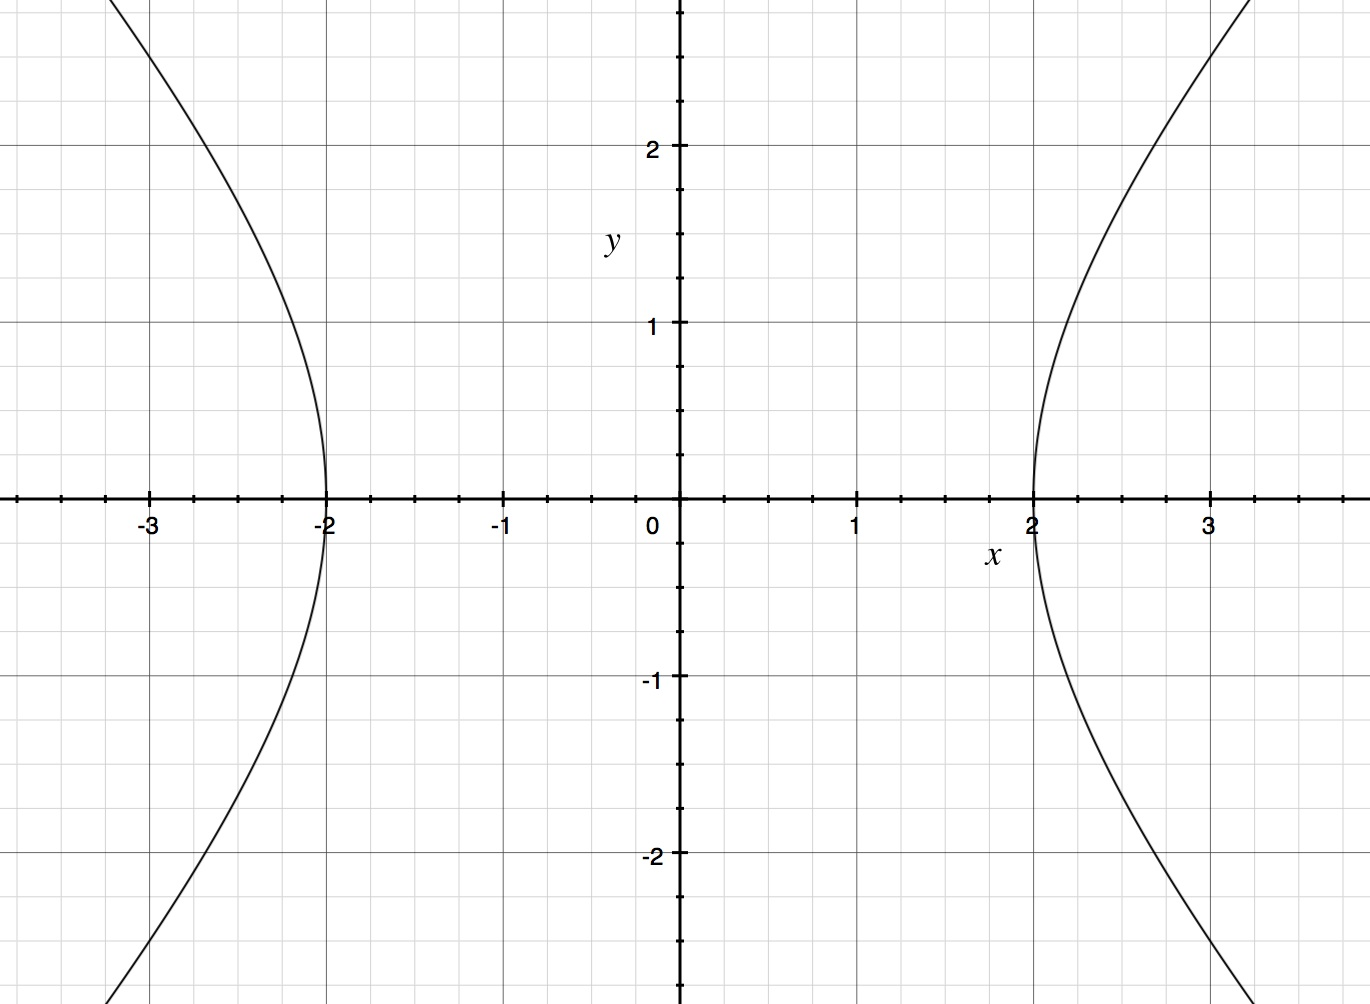
\includegraphics[width=\textwidth]{B.eps}
                \caption{Hyperbola}
                \label{fig:tiger}
        \end{subfigure}
        ~ %add desired spacing between images, e. g. ~, \quad, \qquad etc.
          %(or a blank line to force the subfigure onto a new line)
\end{figure}
\begin{figure}
        \centering
        \begin{subfigure}[b]{0.5\textwidth}
                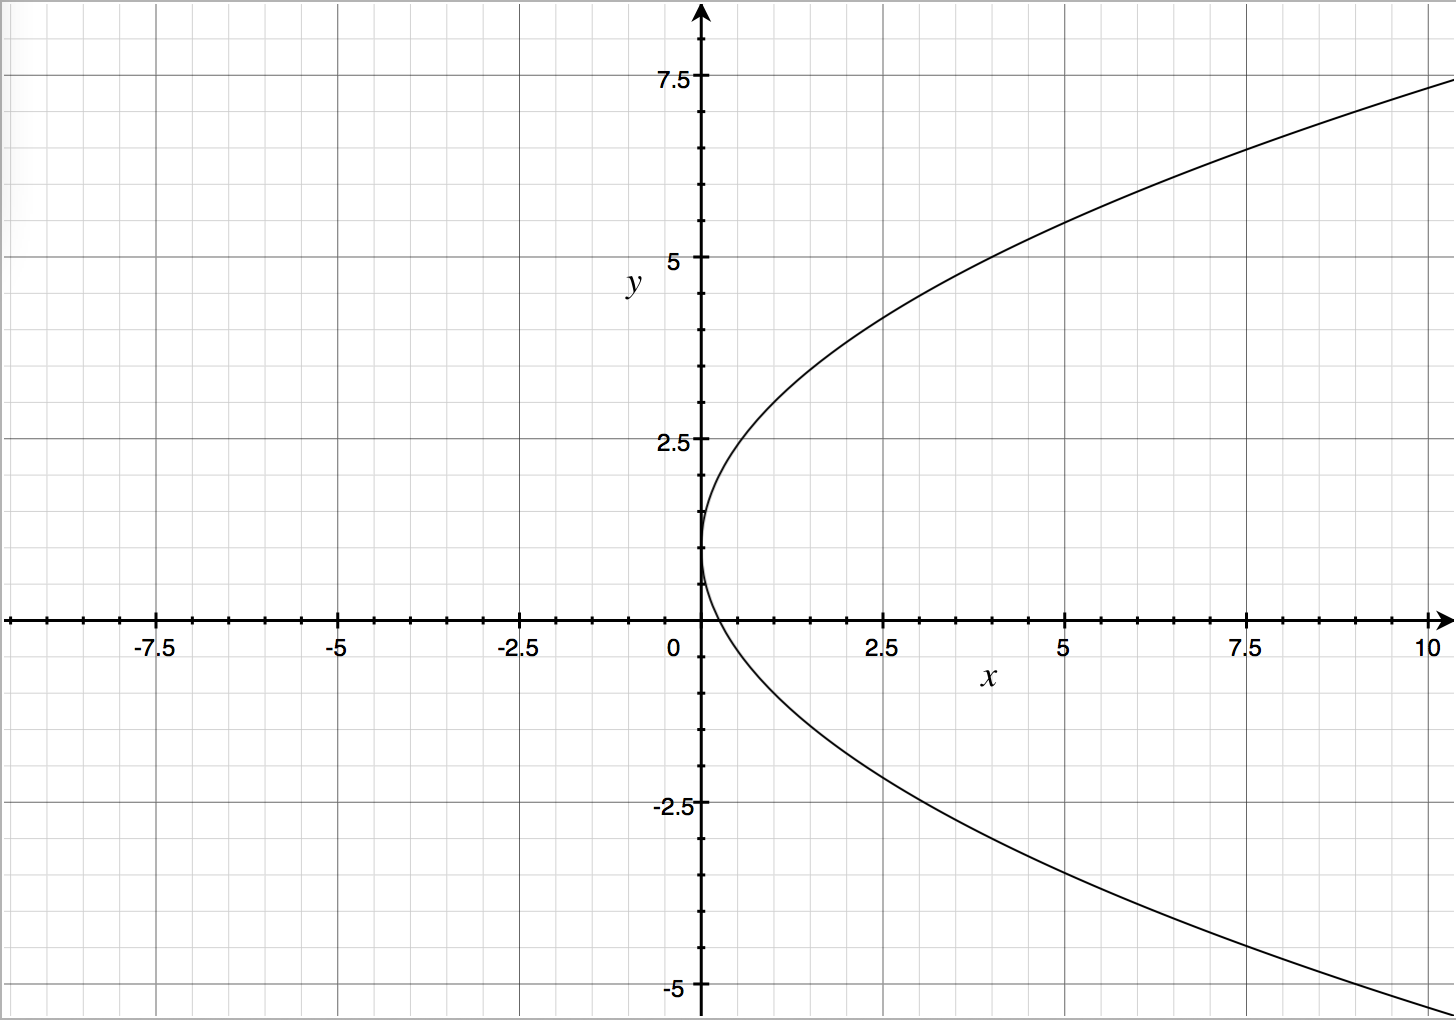
\includegraphics[width=\textwidth]{C.eps}
                \caption{Parabola Centered at $(0,1)$}
                \label{fig:gull}
        \end{subfigure}%
        ~ %add desired spacing between images, e. g. ~, \quad, \qquad etc.
          %(or a blank line to force the subfigure onto a new line)
        \begin{subfigure}[b]{0.5\textwidth}
                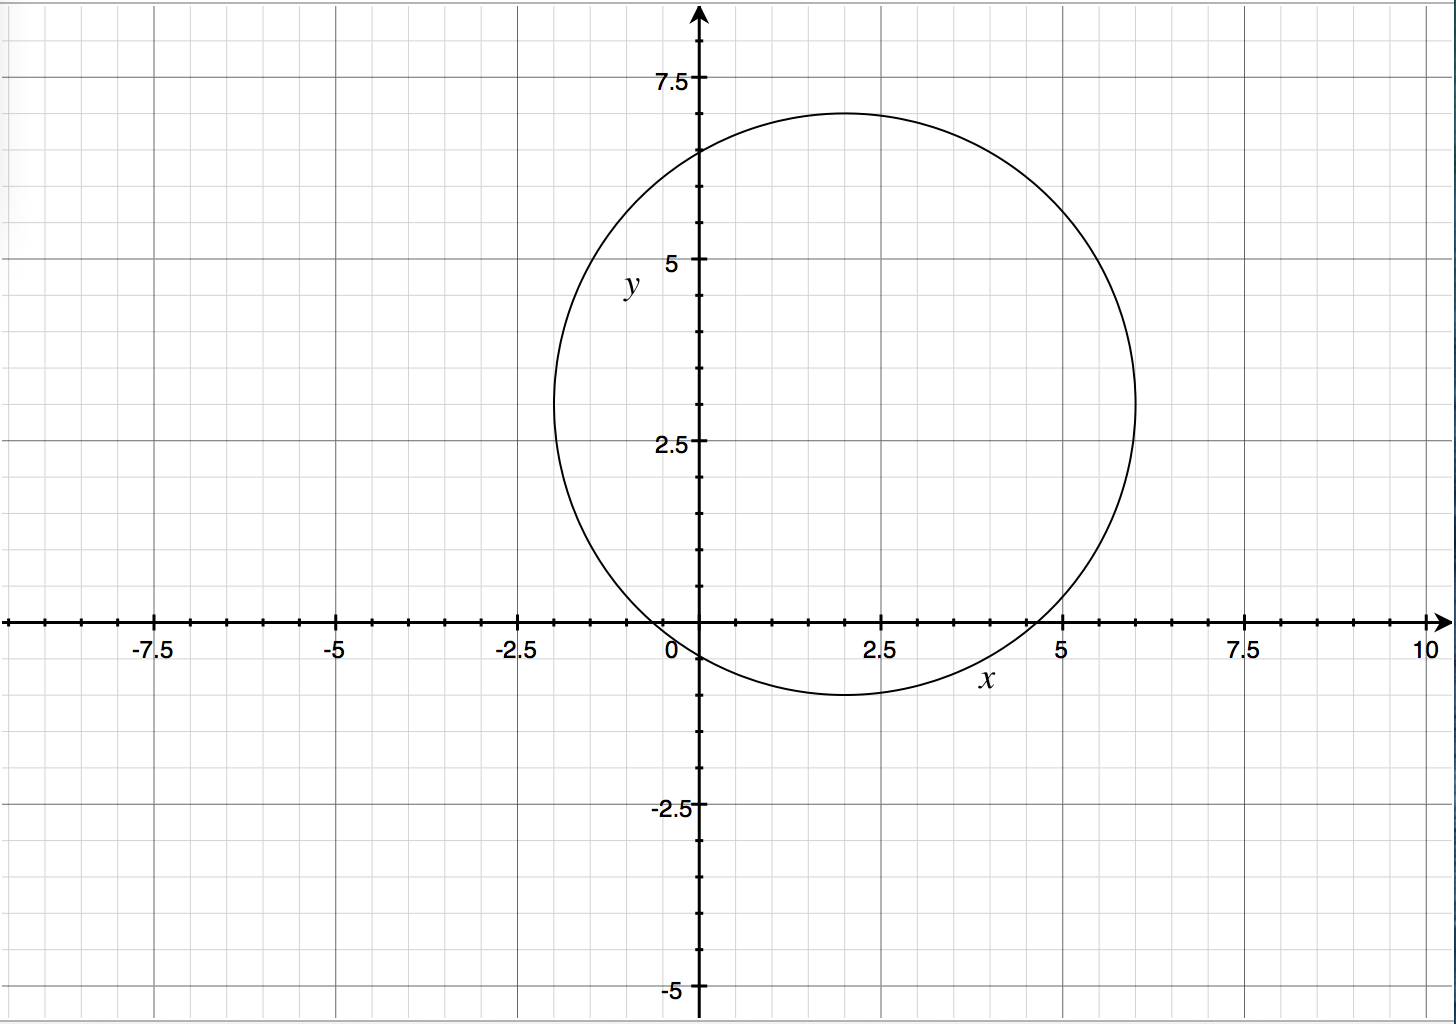
\includegraphics[width=\textwidth]{D.eps}
                \caption{Circle Centered at $(2,3)$}
                \label{fig:tiger}
        \end{subfigure}
        ~ %add desired spacing between images, e. g. ~, \quad, \qquad etc.
          %(or a blank line to force the subfigure onto a new line)
\end{figure}

\end{document}
